\documentclass{llncs}
\usepackage{amssymb}
\usepackage{color}
\usepackage{pgf,pgfarrows,pgfnodes,pgfautomata,pgfheaps,pgfshade}
\usepackage{tikz}
\usetikzlibrary{arrows,decorations.pathmorphing,backgrounds,positioning,fit,petri}
\usepackage{amsmath}

\begin{document}

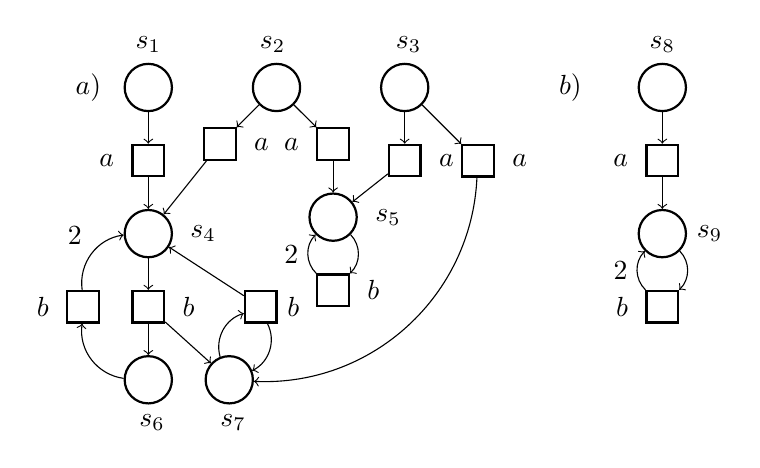
\begin{tikzpicture}[
every place/.style={draw,thick,inner sep=0pt,minimum size=6mm},
every transition/.style={draw,thick,inner sep=0pt,minimum size=4mm},
bend angle=45,
pre/.style={<-,shorten <=1pt,>=stealth,semithick},
post/.style={->,shorten >=1pt,>=stealth,semithick}
]
\def\eofigdist{5.9cm}
\def\eodist{0.4}
\def\eodisty{1}
\def\eodistw{0.7}

\node (a) [label=left:$a) \quad $]{};

\node (q1) [place] [label={above:$s_1$} ] {};
\node (s1) [transition] [below=\eodist of q1,label=left:$a\;$] {};
\node (q2) [place] [right=\eodisty of q1,label=above:$s_2\;$] {};
\node (s2) [transition] [below left=\eodist of q2,label=right:$\;a$] {};
\node (s3) [transition] [below right=\eodist of q2, label=left:$a\;$] {};
\node (q3) [place] [right=\eodisty of q2,label=above:$\;s_3$] {};
\node (s4) [transition] [below =\eodist of q3,label=right:$\;a$] {};
\node (s5) [transition] [below right=\eodistw of q3,label=right:$\;a$] {};

\node (q4) [place] [below=\eodist of s1,label=right:$\;s_4$] {};
\node (q5) [place] [below=\eodist of s3,label=right:$\;s_5$] {};
\node (s6) [transition] [below =\eodist of q4,label=right:$\;b$] {};
\node (s7) [transition] [below =\eodist of q5,label=right:$\;b$] {};
\node (q6) [place] [below=\eodist of s6,label=below:$\;s_6$] {};
\node (s8) [transition] [left =\eodist of s6,label=left:$b\;$] {};

\node (q7) [place] [right=\eodist of q6,label=below:$\;s_7$] {};
\node (s9) [transition] [right =\eodisty of s6,label=right:$b\;$] {};



\draw  [->] (q1) to (s1);
\draw  [->] (q2) to (s2);
\draw  [->] (q2) to (s3);
\draw  [->] (q3) to (s4);
\draw  [->] (q3) to (s5);
\draw  [->] (s1) to (q4);
\draw  [->] (s2) to (q4);
\draw  [->] (s3) to (q5);
\draw  [->] (s4) to (q5);
\draw  [->, bend left] (s5) to (q7);
\draw  [->] (q4) to (s6);
\draw  [->, bend left] (q5) to (s7);
\draw  [->, bend left] (s7) to node[auto] {2} (q5);
\draw  [->] (s6) to  (q6);
\draw  [->, bend left] (q6) to (s8);
\draw  [->, bend left] (s8) to node[auto] {2} (q4);

\draw  [->] (s6) to  (q7);
\draw  [->, bend left] (q7) to (s9);
\draw  [->, bend left] (s9) to (q7);
\draw  [->] (s9) to  (q4);

% seconda rete
  
 
\node (b) [right={5.7cm} of a,label=left:$b)\;\;$] {};

\node (p1) [place]  [right=\eofigdist of q1,label=above:$s_8$] {};
\node (t1) [transition] [below=\eodist of p1,label=left:$a\;$] {};
\node (p2) [place]  [below=\eodist of t1,label=right:$s_9$] {};
\node (t2)  [transition] [below=\eodist of p2,label=left:$b\;$] {};

\draw  [->] (p1) to (t1);
\draw  [->] (t1) to (p2);
\draw  [->, bend left] (p2) to (t2);
\draw  [->, bend left] (t2) to node[auto] {2} (p2);

  
\end{tikzpicture}

\end{document}